% Source: physical PDF p. 244 (printed p. 221). Coverage: complete Figure
% 28.5 and caption. The solid messenger loop, external wavy gauge-superfield
% lines, labels, and the schematic dotted neutral-sector interactions were
% reconstructed from the full-resolution rendered scan.
\begin{figure}[H]
  \centering
  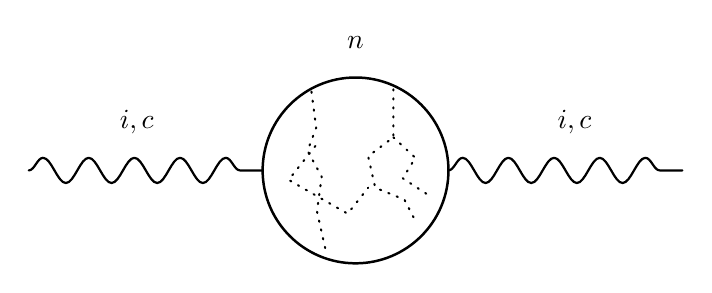
\begin{tikzpicture}[
    x=1cm,
    y=1cm,
    line cap=round,
    line join=round,
    gauge/.style={
      draw,
      line width=0.8pt,
      decorate,
      decoration={snake,amplitude=1.6mm,segment length=5.8mm}
    },
    messenger/.style={draw,line width=0.9pt},
    neutral/.style={
      draw,
      line width=0.75pt,
      dash pattern=on 0.45pt off 2.8pt
    }
  ]
    % Gauge-superfield component lines attached to the messenger loop.
    \draw[gauge] (-4.15,0) -- (-1.18,0);
    \draw[gauge] (1.18,0) -- (4.15,0);
    \node at (-2.78,0.62) {\(\displaystyle i,c\)};
    \node at (2.78,0.62) {\(\displaystyle i,c\)};

    % Messenger component loop.
    \draw[messenger] (0,0) circle[radius=1.18];
    \node at (0,1.62) {\(\displaystyle n\)};

    % Schematic interactions with neutral fields in the
    % supersymmetry-breaking sector.
    \draw[neutral] (-0.56,1.00)
      -- (-0.50,0.54)
      -- (-0.61,0.25)
      -- (-0.43,-0.08)
      -- (-0.49,-0.52)
      -- (-0.38,-1.01);
    \draw[neutral] (0.48,1.03)
      -- (0.48,0.42)
      -- (0.16,0.18)
      -- (0.25,-0.22)
      -- (0.62,-0.37)
      -- (0.77,-0.66);
    \draw[neutral] (-0.51,0.31)
      -- (-0.85,-0.12)
      -- (-0.10,-0.55)
      -- (0.16,-0.22);
    \draw[neutral] (0.48,0.42)
      -- (0.76,0.16)
      -- (0.60,-0.10)
      -- (0.92,-0.31);
  \end{tikzpicture}
  \renewcommand{\thefigure}{28.5}
  \caption{A diagram of the sort that introduces a breakdown of
  supersymmetry into the propagator of the gauge superfields. Here wavy
  lines are any component fields of the gauge superfields; solid lines are
  component fields of the messenger superfields; and dotted lines are
  component fields of the
  \(SU(3)\times SU(2)\times U(1)\)-neutral superfields of
  the supersymmetry-breaking sector.}
  \label{fig:28.5}
\end{figure}
